%
% To make graphic on linux....(require ImageMagic installed)
%
% pdflatex thisfile.tex
% convert -density 300 thisfile.pdf -resize 640x480 thatfile.png 
%
% On Windows 10.... copy ImageMagic's convert.exe to your path 
% or rename it imgconvert.exe
% Get recent version of GhostScript
%
% pdflatex thisfile.tex
% convert -density 300 thisfile.pdf -resize 640x480 thatfile.png 
%
% Trouble? See this thread
%
% https://tex.stackexchange.com/questions/11866/compile-a-latex-document-into-a-png-image-thats-as-short-as-possible/11880#11880
%
\documentclass{standalone}
\usepackage{tikz}

\author{CC-BY-2016 James B. Wilson}
\date{2016}
\date{today}
\begin{document}
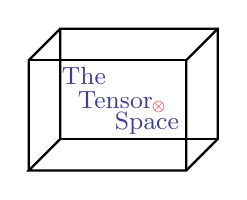
\begin{tikzpicture}[scale=.2]
\draw[thick] (0,2) -- (0,9) -- (10,9) -- (10,2) -- (8,0) -- (-2,0) -- (0,2);
\draw[thick] (-2,0) -- (-2,7) -- (0,9);
\draw[thick] (8,0) -- (8,7) -- (10,9);
\draw[thick] (-2,7) -- (8,7);
\draw[thick] (0,2) -- (10,2);
\node[text=black!60!blue!75] at (1.5,6) {\small The};
\node[text=black!60!blue!75] at (3.5,4.5) {\small Tensor};
\node[text=red!80] at (6.25,4) {\tiny $\otimes$};
\node[text=black!60!blue!75] at (5.5,3){\small Space};
\end{tikzpicture}
\end{document}
